% !TeX spellcheck = cs_CZ
%{\tikzset{external/prefix={tikz/FYZII/}}
% \tikzset{external/figure name/.add={ch16_}{}}
%---------------------------------------------------------------------------------------------------
% file fey2ch16.tex
%---------------------------------------------------------------------------------------------------
%====================Kapitola: Indukované proudy ===================================================
\setchaptertoc
\chapter{Indukované proudy}\label{fyz:IIchapXVI}


\section{Motory a generátory}\label{fyz:IIchapXVIsecI}


\section{Transformátory a indukčnosti}\label{fyz:IIchapXVIsecII}

  
\section{Síly působící na indukované proudy}\label{fyz:IIchapXVIsecIII}


\section{Elektrotechnika}\label{fyz:IIchapXVIsecIV}

  \begin{figure}[ht!]  %\ref{fyz:fig0311}
    \centering
    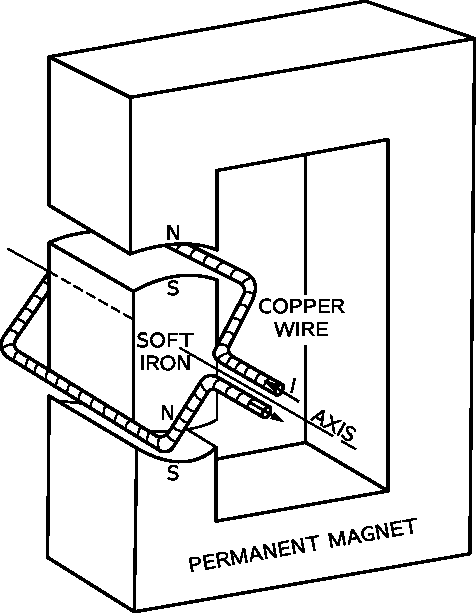
\includegraphics[width=0.8\linewidth]{fyz_fig0311.pdf}
    \caption{
             (\cite[s.~148]{Feynman02}).}
    \label{fyz:fig0311}
  \end{figure}

  \begin{figure}[ht!]  %\ref{fyz:fig0312}
    \centering
    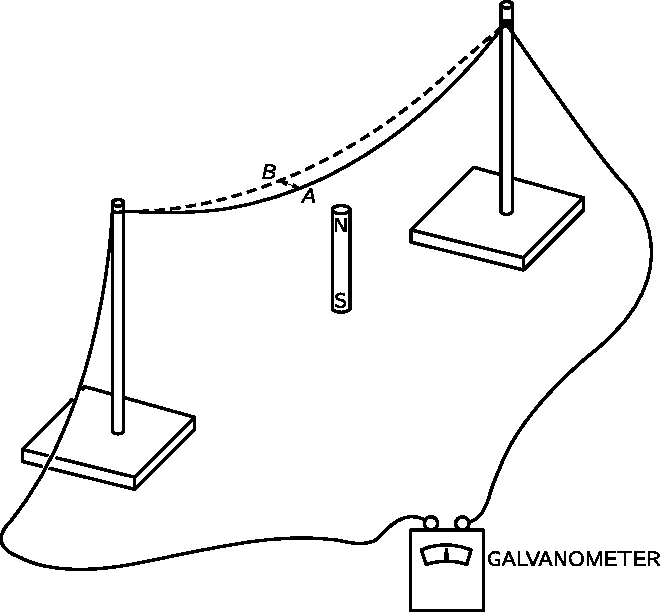
\includegraphics[width=0.8\linewidth]{fyz_fig0312.pdf}
    \caption{
             (\cite[s.~148]{Feynman02}).}
    \label{fyz:fig0312}
  \end{figure}

  \begin{figure}[ht!]  %\ref{fyz:fig0313}
    \centering
    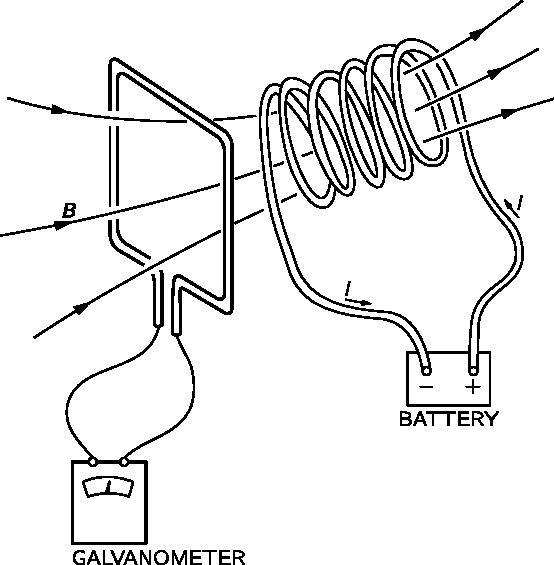
\includegraphics[width=0.8\linewidth]{fyz_fig0313.pdf}
    \caption{
             (\cite[s.~148]{Feynman02}).}
    \label{fyz:fig0313}
  \end{figure}

  \begin{figure}[ht!]  %\ref{fyz:fig0314}
    \centering
    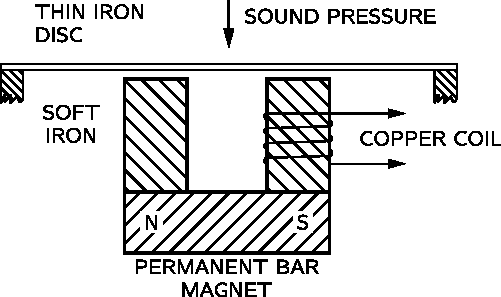
\includegraphics[width=0.8\linewidth]{fyz_fig0314.pdf}
    \caption{
             (\cite[s.~148]{Feynman02}).}
    \label{fyz:fig0314}
  \end{figure}

  \begin{figure}[ht!]  %\ref{fyz:fig0315}
    \centering
    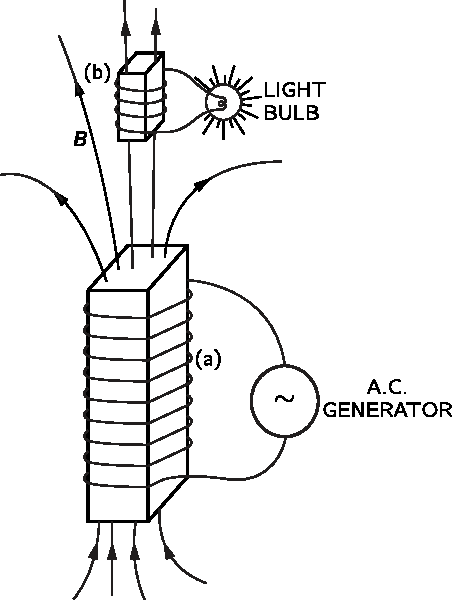
\includegraphics[width=0.8\linewidth]{fyz_fig0315.pdf}
    \caption{
             (\cite[s.~148]{Feynman02}).}
    \label{fyz:fig0315}
  \end{figure}

  \begin{figure}[ht!]  %\ref{fyz:fig0316}
    \centering
    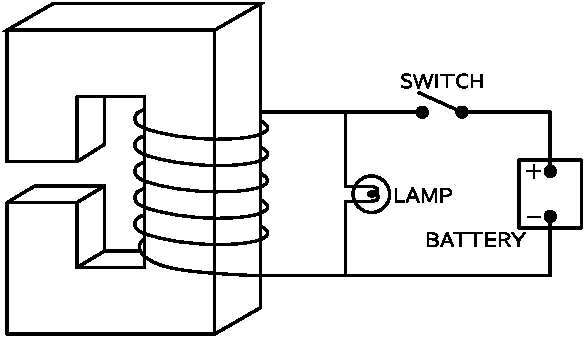
\includegraphics[width=0.8\linewidth]{fyz_fig0316.pdf}
    \caption{
             (\cite[s.~148]{Feynman02}).}
    \label{fyz:fig0316}
  \end{figure}
  
  \begin{figure}[ht!]  %\ref{fyz:fig0317}
    \centering
    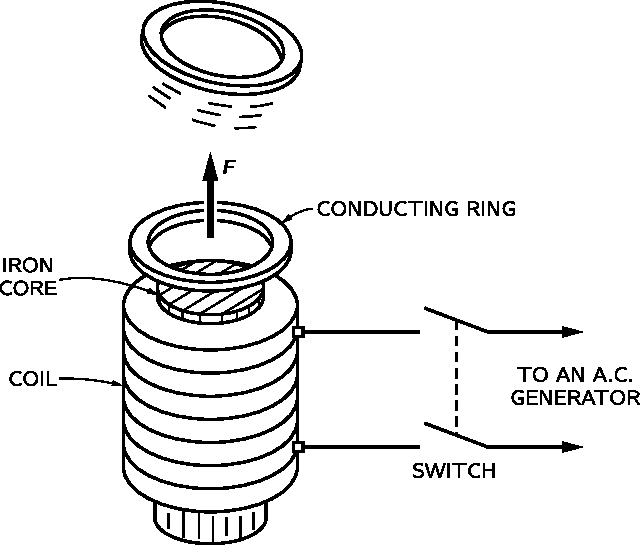
\includegraphics[width=0.8\linewidth]{fyz_fig0317.pdf}
    \caption{
             (\cite[s.~148]{Feynman02}).}
    \label{fyz:fig0317}
  \end{figure}

  \begin{figure}[ht!]  %\ref{fyz:fig0318}
    \centering
    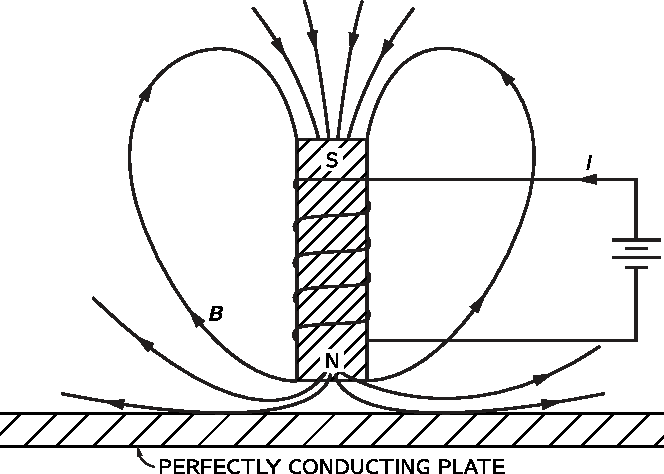
\includegraphics[width=0.8\linewidth]{fyz_fig0318.pdf}
    \caption{
             (\cite[s.~148]{Feynman02}).}
    \label{fyz:fig0318}
  \end{figure}

  \begin{figure}[ht!]  %\ref{fyz:fig0319}
    \centering
    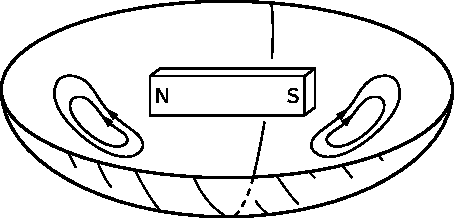
\includegraphics[width=0.8\linewidth]{fyz_fig0319.pdf}
    \caption{
             (\cite[s.~148]{Feynman02}).}
    \label{fyz:fig0319}
  \end{figure}

  \begin{figure}[ht!]  %\ref{fyz:fig0320}
    \centering
    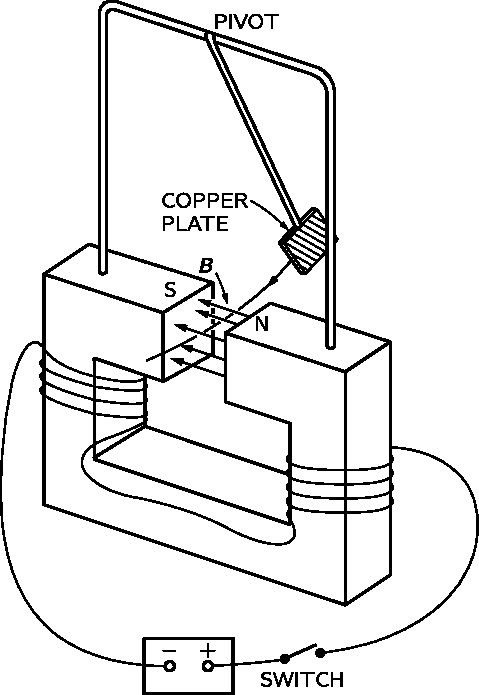
\includegraphics[width=0.8\linewidth]{fyz_fig0320.pdf}
    \caption{
             (\cite[s.~148]{Feynman02}).}
    \label{fyz:fig0320}
  \end{figure}

  \begin{figure}[ht!]  %\ref{fyz:fig0321}
    \centering
    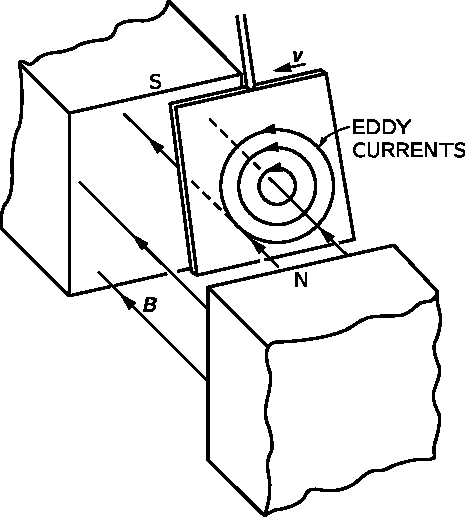
\includegraphics[width=0.8\linewidth]{fyz_fig0321.pdf}
    \caption{
             (\cite[s.~148]{Feynman02}).}
    \label{fyz:fig0321}
  \end{figure}

  \begin{figure}[ht!]  %\ref{fyz:fig0322}
    \centering
    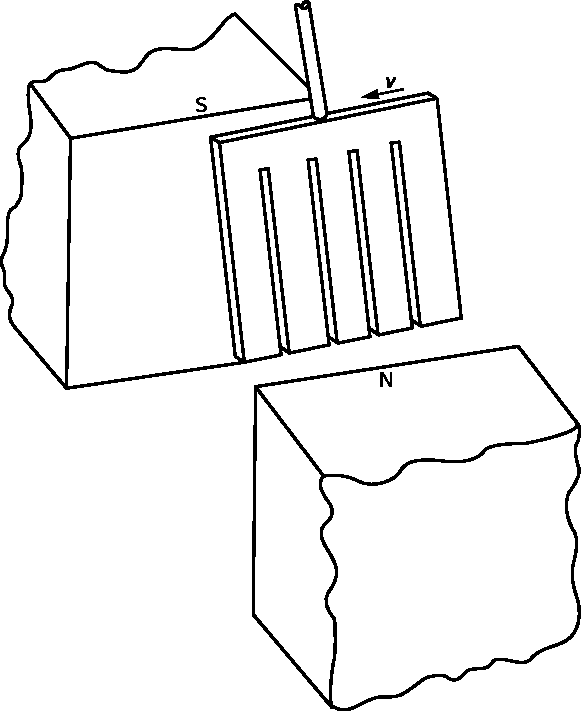
\includegraphics[width=0.8\linewidth]{fyz_fig0322.pdf}
    \caption{
             (\cite[s.~148]{Feynman02}).}
    \label{fyz:fig0322}
  \end{figure}
  
  \begin{figure}[ht!]  %\ref{fyz:fig0323}
    \centering
    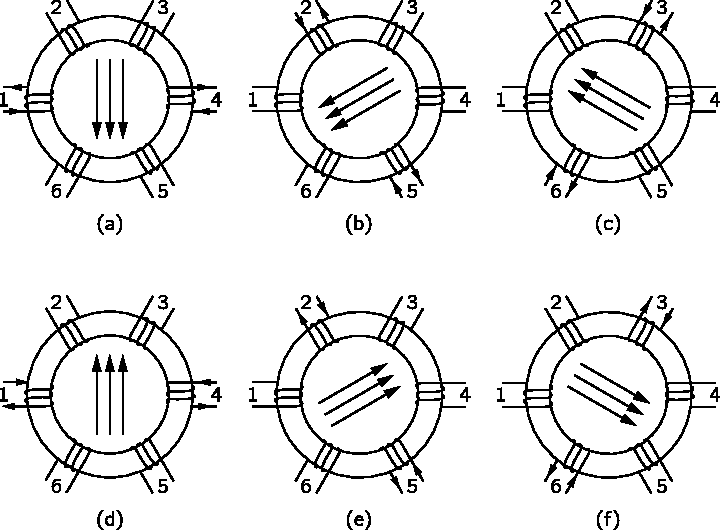
\includegraphics[width=0.8\linewidth]{fyz_fig0323.pdf}
    \caption{
             (\cite[s.~148]{Feynman02}).}
    \label{fyz:fig0323}
  \end{figure}
  
  \begin{figure}[ht!]  %\ref{fyz:fig0324}
    \centering
    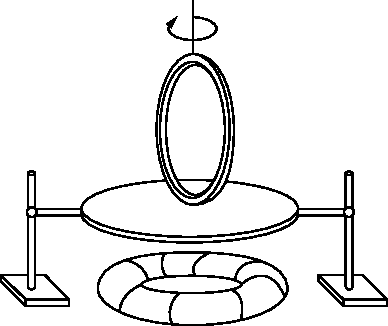
\includegraphics[width=0.8\linewidth]{fyz_fig0324.pdf}
    \caption{
             (\cite[s.~148]{Feynman02}).}
    \label{fyz:fig0324}
  \end{figure}

  \begin{figure}[hb!]
    \centering
    \subcaptionbox{\label{fyz:fig0325a}}{\luafigure[0.45]{fyz_fig0325a.pdf}}
    \subcaptionbox{\label{fyz:fig0325b}}{\luafigure[0.45]{fyz_fig0325b.pdf}}
    \caption{ }
    \label{fyz:fig0325}
  \end{figure}

  \todo[inline]{Kapitola fey2ch16 je nedodělaná, obsahuje pouze obrázky}
%} %tikzset
%~~~~~~~~~~~~~~~~~~~~~~~~~~~~~~~~~~~~~~~~~~~~~~~~~~~~~~~~~~~~~~~~~~~~~~~~~~~~~~~~~~~~~~~~~~~~~~~~~~
